\documentclass[12pt,a4paper]{article}
%-----------------------PACKAGES-----------------------%
\usepackage[top=1in,bottom=1in,left=0.5in,right=0.5in]{geometry}
\usepackage{graphicx}
\usepackage{array}
\usepackage{xcolor}
\usepackage{adjustbox}
\usepackage{titlesec}
\usepackage{svg}
\usepackage{lettrine}

%-----------------------TABLES ALIGNEMNET-----------------------%

%-----------------------TITLE DOCUMENT-----------------------%
\begin{document}
	\begin{Titlepage}
\begin{center}
    \vspace*{2cm}
    
    \textbf{\Large  Data Mining Project}\\
    \vspace*{2cm}
      \begin{center}
          \large M.Wahaj Tahir\\F191014@cfd.nu.edu.pk\\wahajt@acm.org
      \end{center} 
    
    \vspace{1.5cm}
    
    \vspace{0.3cm}
    \begin{center}
           \large April,2023
      \end{center}
    \vfill
    \vspace{0.8cm}
    \begin{figure}[hb]
        \centering
        
\includegraphics[scale=0.20]{Fast-Nuces.png}
    \end{figure}
    

     Department of Computer Science\\ National University of Computer and Emerging Science\\ Chiniot Faisalabad Campus, Pakistan 2023
    \end{center}

\end{Titlepage}
 
 \clearpage
%-----------------------TABLE OF CONTENT-----------------------% 
\tableofcontents
\clearpage
%-----------------------TABLE OF CONTENT-----------------------% 
\section{Exploratory Data Analysis}
The dataset which  is provided to us is in excel format and it consist of 7 sheets in it.I’m assuming these different sheets are representing different courses and different student are enrolled in these courses. I have loaded these sheets in different data frames and these are the common data dictionary(columns) I have found.
\subsection{Data Dictionary}
A data dictionary is a type of dictionary that tells us what type of data is describing itself.
\begin{table}[h!]
\caption{Data Dictionary}
    \centering
    \begin{tabular}{|p{3cm}|p{3cm}|p{5cm}|}
    \hline
       \textbf{Dictionary}&Data Type&\textbf{Description} \\ %end of row
       \hline
        \textbf{As:1,..,6}&Float64&The marks  of assignments of each student in a particular assignment. \\ %end of row
        \hline
         \textbf{As}&Float64&The total number obtained from all assignments. \\ %end of row
        \hline
        \textbf{Qz:1,..,6}&Float64&The marks of quizzes of each student in a particular  Quiz. \\ %end of row
        \hline
         \textbf{Qz}&Float64&The total number obtained from all quizzes. \\ %end of row
        \hline
         \textbf{S-I}&Float64&The exam marks of individual from total. \\ %end of row
        \hline
        \textbf{S-II}&Float64&The Mid-exam marks of individual from total \\ %end of row
        \hline
        \textbf{Grade}&Object&Either the student is pass or fail in that particular subject \\ %end of row
        \hline      
    \end{tabular} 
    \end{table}
\newline The given table is telling us what each column is telling about the data.
\subsection{Data Pre-processing}
I loaded these files \textbf{jupyter note book} and start working on it and check ambiguities in the Excel file and did some pre-processing on it and found some errors. Which can be found in the given code.\par
After doing this, I tried to understand the data and found \textbf{Mean},\textbf{Median},\textbf{Mode},\textbf{Min},\textbf{Max},\textbf{total counts etc}, after that I found out the total number of null values. By looking at the data there are not many null values that can affect the model training.I thought of changing the \textbf{NAN} value with zero. After that, I did some drawn histograms of each sheet and displayed the data which is giving the information about each course.
\newpage
\subsection{Data Visualization:}
The data is Visualized.
\begin{figure}[h]
    \centering
    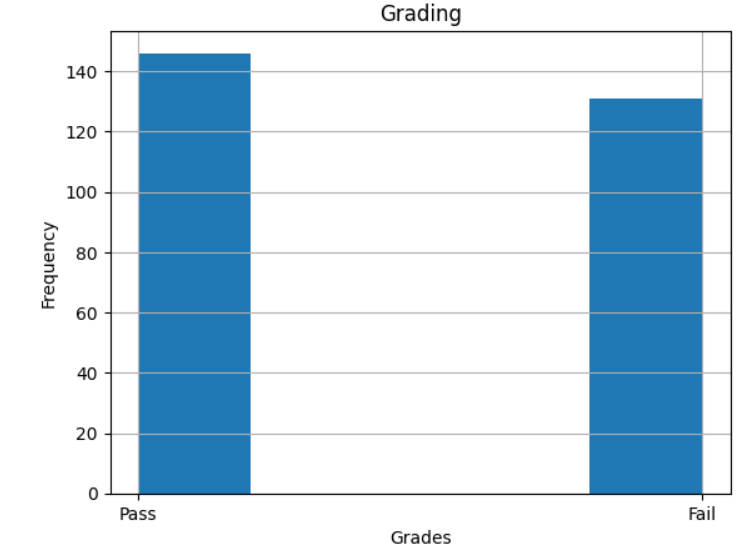
\includegraphics[scale=0.60]{Other/Grading.png}
    \caption{Grading}
\end{figure}
\newline In order to find the basic information regarding each attribute in our dataset we used the “describe” function provided by pandas.
\begin{figure}[h]
    \centering
    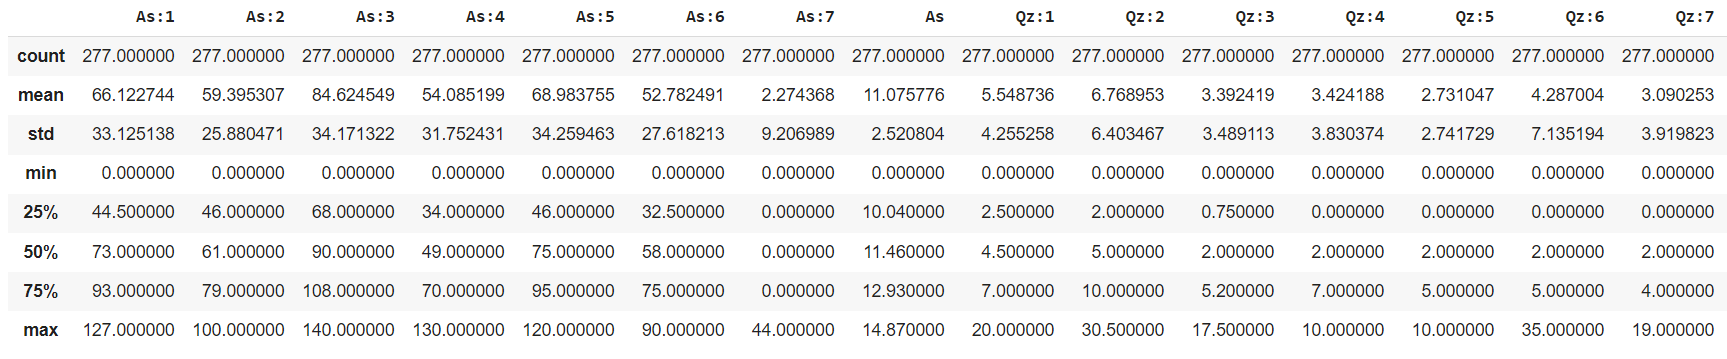
\includegraphics[scale=0.40]{Other/Data_Dictonary.png}
    \caption{Data Description}
\end{figure}
\newpage
\newline Next on we checked which assignments and quizzes contained most students with zero marks.
\begin{figure}[h]
    \centering
    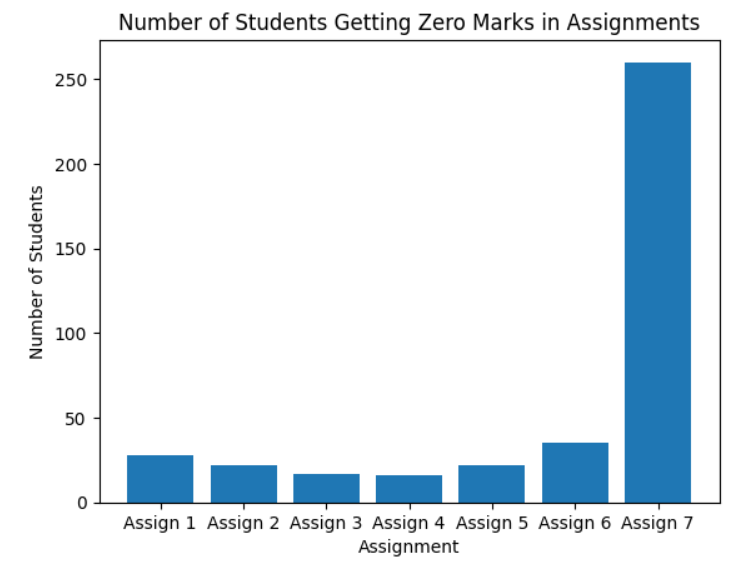
\includegraphics[scale=0.50]{Other/Assignment.png}
    \caption{Assignment}
\end{figure}

\begin{figure}[h]
    \centering
    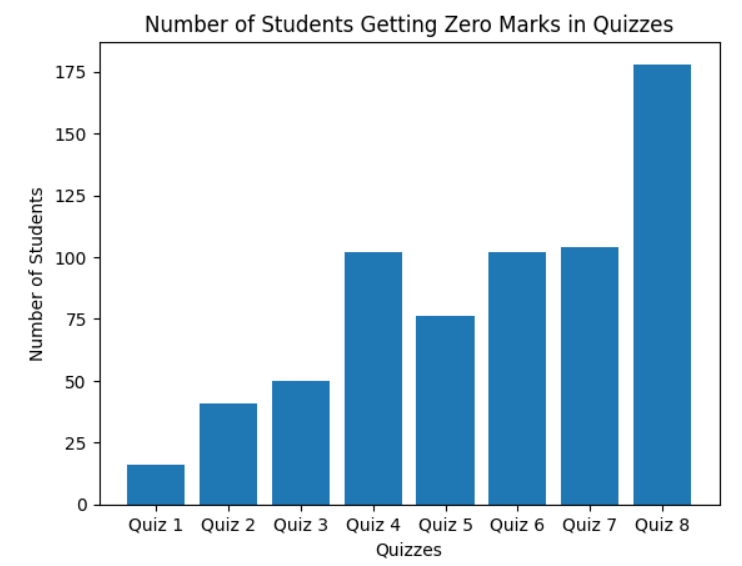
\includegraphics[scale=0.50]{Other/Quizzes.png}
    \caption{Quizes}
\end{figure}
\newpage
To get an idea of how the assignments, quizzes and exams are related to each other we used the correlation matrix. 
\begin{figure}[h]
    \centering
    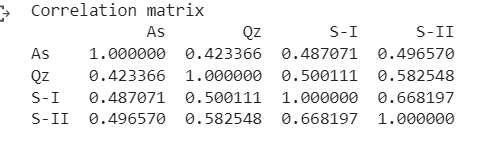
\includegraphics[scale=0.60]{Other/correlation_matrix.png}
    \caption{Correlation matrix}
\end{figure}
The results show that all of them are positively correlated, which means if a student is doing good in assignments and quizzes it is more likely that they will be successful in exams.
\subsection{Modeling Training and Testing}
For all the models we used 80\% of the data for training and the remaining 20\% for testing. We also extracted the basic measuring values for each model.
\subsection{KNN}
KNN is one of the most common models used in industrial problems. We used the first four assignments and quizzes, and the Mid I exams as features. The ‘Grade’ column served as the target.  
\newline Our model was giving the following figures when we applied the measuring metrics to our model.
\begin{figure}[h]
    \centering
    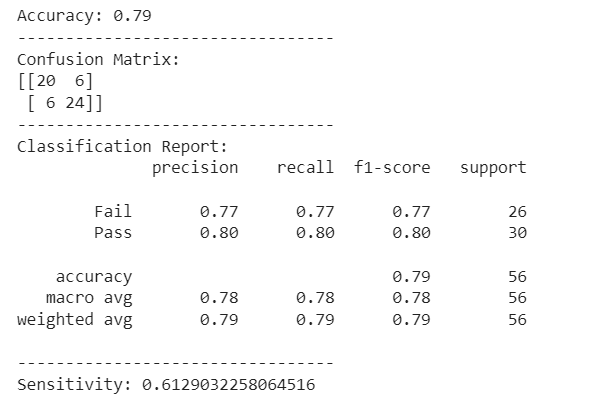
\includegraphics[scale=0.60]{Other/KNN_Model.png}
    \caption{KNN}
\end{figure}
\newpage
\subsection{Decision Tree}
Our Decision Tree Classifier was giving the following figures when we applied the measuring metrics to it.
\begin{figure}[h]
    \centering
    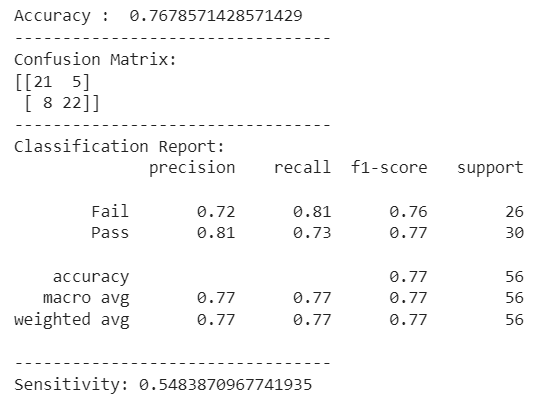
\includegraphics[scale=0.60]{Other/Decision_tree.png}
    \caption{Decision tree}
\end{figure}


\subsection{Naive Bayes}
Our Naïve Bayes model was giving the following figures when we applied the measuring metrics to it.
\begin{figure}[h]
    \centering
    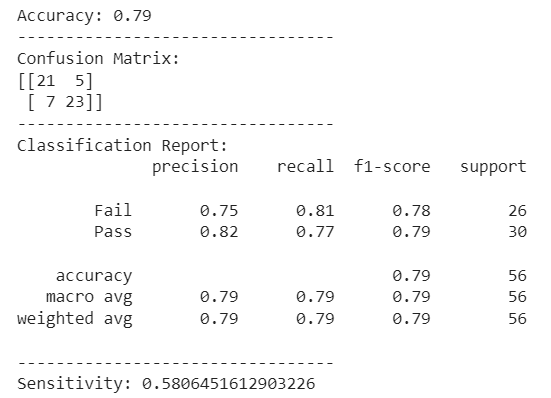
\includegraphics[scale=0.60]{Other/Naive_Baiyesin.png}
    \caption{Naive Bayes}
\end{figure}


\newpage
\section{After Results}
\subsection{KNN}
\begin{figure}[h]
    \centering
    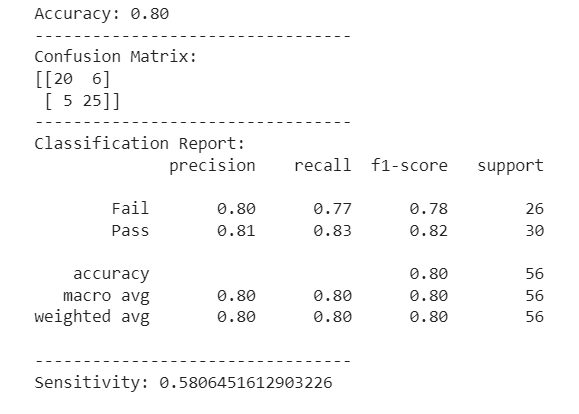
\includegraphics[scale=0.60]{Other/After_KNN.png}
    \caption{KNN}
\end{figure}
\subsection{Decision Tree}
\begin{figure}[h]
    \centering
    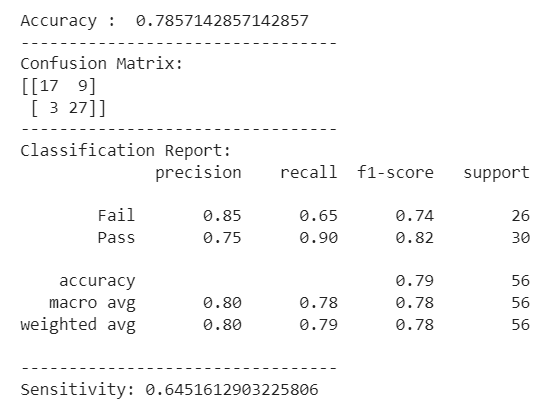
\includegraphics[scale=0.60]{Other/After_Decision Tree.png}
    \caption{Decision tree}
\end{figure}
\newpage
\subsection{Naive Bayes}
\begin{figure}[h]
    \centering
    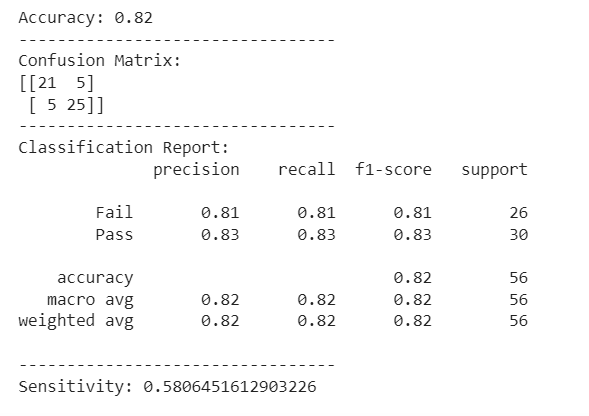
\includegraphics[scale=0.60]{Other/After_Bayesian.png}
    \caption{Naive Bayes}
\end{figure}


\end{document}